\documentclass[conference]{IEEEtran}
\usepackage[T1]{fontenc}
\usepackage{mathptmx}
\usepackage{amsmath,amssymb,booktabs,graphicx,url}
\usepackage{balance}
\usepackage[hidelinks]{hyperref}
\newtheorem{theorem}{Theorem}
\newtheorem{proposition}[theorem]{Proposition}
\newtheorem{lemma}[theorem]{Lemma}
\newcommand{\stable}{\textsf{STABLE}}
\newcommand{\unstable}{\textsf{UNSTABLE}}
\newcommand{\unknown}{\textsf{UNKNOWN}}
\newcommand{\one}{\boldsymbol{1}}
\newcommand{\norm}[1]{\left\lVert#1\right\rVert_1}
\title{ViewRank: Certifying Top-k Stability over Local Graph Policy Domains}
\author{\IEEEauthorblockN{Wenji Fu}
\IEEEauthorblockA{Southwestern University of Finance and Economics\\
fuwenji61616@gmail.com\\
\href{https://orcid.org/0009-0003-7757-140X}{ORCID: 0009-0003-7757-140X}}}
\begin{document}
\maketitle
\begin{abstract}
Auditing a registered batch of graph retrieval requests requires deciding whether the same top-$k$ evidence set persists throughout a continuous range of relation weights. Point samples cannot establish this statement, while independent source-wise bounds can lose the dependence imposed by shared weights. We present ViewRank, an execution operator for top-$k$ stability over local graph policy domains. Moving source normalizers into the unknowns exposes an affine system on the $r$ modified sources. Its determinant clears every score comparison to a polynomial of total degree at most $r$. An a posteriori certificate combines approximate graph responses, source interactions, and omitted-coordinate tails in this polynomial representation, covering every policy and every output node. A budgeted directory reuses responses and retains output coordinates selected from the current query. On 3,417 fixed HotpotQA and MuSiQue questions, three paired blocks reduce complete-workload cost by 34.7--35.3\% and 65.9--66.0\%, respectively, against source-wise lifting with the same compressed representation, while resolving more complete audits. Pruned full-response execution with the same certificate exposes complementary time and coverage tradeoffs. In a separate witness-free capacity study at 1\,MiB, compressed retention certifies all three cutoffs stable for 51.0\%/63.1\% of original questions, versus 0\%/53.5\% with pruned full responses. Whole-domain proof replay covers all 9,674 distinct primary stable question--cutoff pairs; independent full-response audits check numerical premises on 52 representative responses, and cold solves validate actual instability witnesses. Shared-core SMT and propagation-strength studies further characterize verification and execution boundaries. ViewRank makes continuous policy auditing practical by connecting source-local compilation to approximate numerical execution and whole-output certification.
\end{abstract}

\section{Introduction}
A graph retrieval policy determines how relations carry evidence. Consider an analyst auditing a batch of retrieval requests before exposing their evidence sets to downstream consumers. For each request, the analyst specifies how much mention links and weaker associations may be reweighted at the named sources. The useful request is: \emph{does the same top-$k$ evidence set remain valid for every pair of weights in that range?} A stable set can be reused by membership-only consumers throughout the range, avoiding further point-policy searches for a replacement set. An instability witness gives two settings for inspecting the replacement, fixing a policy, or revising the permitted range. Scores and within-set order may still vary.

The rectangle is an analyst input. Local source selection models a query-specific intervention on the entities through which that request enters the graph; background relations stay fixed. Reweighting all graph sources is a different intervention, for which the small-source specialization need not remain efficient. Our implementation evaluates registered batch audits, with registration reading source identifiers only. This contract concerns evidence membership and does not itself establish answer accuracy.

A concrete audit concerns a HotpotQA question about the fanzine that interviewed the Sex Pistols bassist during his time in The Flowers of Romance~\cite{hotpot}. Two legal settings replace Ex Pistols by Sid Vicious in top-2, bringing both annotated supporting passages into the retrieved set (Fig.~\ref{fig:operator}). Strict actual-view certificates establish this policy sensitivity. The corresponding universal question asks whether such a change occurs anywhere in the declared weight rectangle, rather than only at settings an auditor happens to try.

Ranking sensitivity under uncertain weights and stable top-$k$ regions have established database foundations~\cite{uncertainranking,stablerankings}. The present request brings them to normalized graph propagation executed with approximate responses. It changes the unit of execution from a point policy to a continuous domain. Efficient personalized PageRank (PPR) solving~\cite{maehara}, edge-weight model reduction~\cite{edgeppr}, and incremental propagation~\cite{osp,eveppr} provide strong foundations for a particular policy. Evaluating a grid supplies observations, but an interior policy can change membership even when every global corner agrees. Parametric verification supplies sound regional techniques~\cite{parametric,lifting,sapo}; a source-wise relaxation can nevertheless admit combinations that no common pair of policy weights produces. The execution problem is to establish a universal output statement while retaining the dependence that makes it provable.

We exploit the locality of the change. Suppose the policy modifies outgoing distributions at $r$ sources, using two global relation weights and a fixed self-loop group. At most $2r$ signed graph responses capture the changes. Moving each column normalizer into its source variable leaves an $r\times r$ system whose entries are affine in the two weights. Clearing its determinant converts every score comparison into a polynomial of total degree at most $r$. The symbolic dimension follows the modified sources, while graph-dependent preparation remains numerical. In our natural workloads $r\leq4$; the algebraic statement does not require this extractor bound.

The second observation concerns the output. A ranking audit must separate the requested nodes from \emph{all} alternatives, but need not reconstruct every response coordinate at every policy. ViewRank retains source interactions and selected output rows. Algebraic cancellation of the source update expresses solver error in the same determinant-cleared coefficients, avoiding a separate inverse-source-core error bound. Coordinate tails cover every omitted entry. These allowances use the same policy variables as the score numerators. A coefficient test then covers both the candidate boundary and every node outside the candidate scan throughout the domain. The approximate determinant is separately checked for positivity; positivity of the exact physical determinant is not transferred to an approximate system.

The central contribution is the a posteriori connection in Eqs.~\eqref{eq:cancellation}--\eqref{eq:certificate}. Coherent source interactions cancel the source update in the residual equation, letting approximate-response errors enter the same determinant-cleared functions as the scores. Coordinate tails extend the certificate to retained candidates and every omitted competitor. The affine source compiler exposes this structure, while a budgeted executor makes the responses reusable across a registered workload. Low-rank elimination, ranking stability, Bernstein bounds, and caching supply established building blocks; their combination here yields a whole-domain membership proof from approximate, partially retained graph responses.

We compare the complete operator with strong source-wise lifting and an atom-free single-source path, and compressed retention with pruned full responses using the same polynomial certificate. We report total cost, tail latency, coverage, retained state, and separate operating-system memory.

Across the complete 1,000-question HotpotQA and 2,417-question MuSiQue traces, the sparse operator resolves all cutoffs for 997 and 2,392 questions. Against lifting with the same compressed retention, it lowers complete-workload cost by 34.7--35.3\% and 65.9--66.0\% in every paired block while resolving five and 22 additional complete audits. Every original request remains in the comparison.

\begin{figure}[t]
\centering
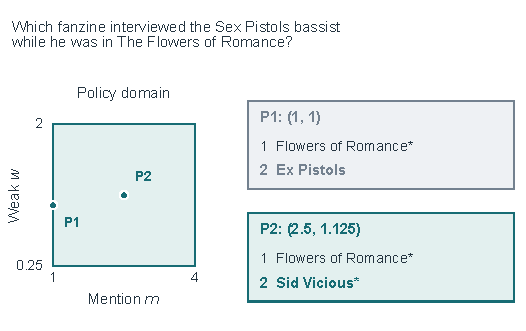
\includegraphics[width=\columnwidth]{../figures/domain_example.pdf}
\caption{A real policy-sensitive retrieval. Two points in the legal rectangle return different top-2 sets, with strict true boundary-gap lower bounds $1.229\times10^{-5}$ and $5.370\times10^{-5}$. Stars mark annotated supporting passages, used post hoc to select and explain this positive illustration.}
\label{fig:operator}
\end{figure}

\section{Policy-Domain Query}
\label{sec:problem}
Let $P_0$ be a nonnegative column-stochastic transition matrix, $h\geq0$ a fixed seed with $\one^Th=1$, and $0<\alpha<1$. Columns are source distributions. A query modifies the complete outgoing distributions of its original sources $S=(s_1,\ldots,s_r)$. At source $s$, mention and weak-link subdistributions $g_{m,s},g_{w,s}\geq0$ and the self-loop partition the original column:
\begin{equation}
 P_0[:,s]=g_{m,s}+g_{w,s}+p_{ss}e_s,\quad
 \mu_s+\nu_s+p_{ss}=1,
 \label{eq:partition}
\end{equation}
where $\mu_s=\one^Tg_{m,s}$ and $\nu_s=\one^Tg_{w,s}$. Common positive weights $\theta=(m,w)$ define
\begin{equation}
 \begin{aligned}
 P_\theta[:,s]&=\frac{m g_{m,s}+w g_{w,s}+p_{ss}e_s}{Z_s},\\
 Z_s&=1+(m-1)\mu_s+(w-1)\nu_s.
 \end{aligned}
 \label{eq:policy}
\end{equation}
All other columns are fixed. Scores are $x(\theta)=A_\theta^{-1}b$, with $A_\theta=I-\alpha P_\theta$ and $b=(1-\alpha)h$. Stochasticity ensures existence, nonnegativity, and unit total score. Section~\ref{sec:raw} extends the contract to stored graph columns whose exact sums differ slightly from one.

A domain query supplies a closed rectangle $\Theta=[m_-,m_+]\times[w_-,w_+]$ bounded away from zero and one or more cutoffs $k$. For each cutoff, \stable\ returns a size-$k$ membership and certifies it for every $\theta\in\Theta$. \unstable\ returns two in-domain policies with independently certified, strictly separated top-$k$ memberships that differ. \unknown\ means neither conclusion has been established within the allowed work. Identifiers break exact ranking ties, but a strict-separation certificate may remain unresolved at such a boundary. Stability permits scores and within-set order to change. A top-10 certificate alone establishes neither top-2 nor top-5 stability.

The weights are audit inputs, rather than parameters learned from support labels. The fixed seed and original sources remain unchanged throughout the domain. Questions may reuse sources and responses, but each remains a separate query with its own seed and requested outputs.

Effective dimension depends on the partition. If all modified sources have zero self mass, common scaling of $(m,w)$ cancels and the view depends only on $m/w$. Disjoint mention/weak/self supports all positive at one source give two independent policy directions. Sources with only two positive groups each contribute one direction; different direction types across sources can jointly give dimension two. We audit this structure on the stored input.

Figure~\ref{fig:overview} connects the query contract to its execution. Seed-independent graph responses enter a budgeted directory. A query combines their source interactions with its base ranking to compile a small affine system; retained rows, residuals, and tails then support the whole-output test. A successful cover returns \stable. An unresolved test can invoke actual-policy solves to find a strict \unstable\ witness, or finish \unknown\ within the declared work.

\begin{figure}[t]
\centering
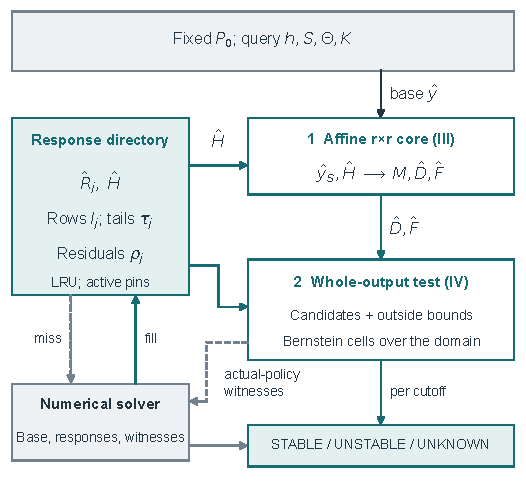
\includegraphics[width=\columnwidth]{../figures/domain_overview.pdf}
\caption{ViewRank overview. Reusable responses supply the affine source compiler and the whole-output test. Solid arrows carry data/results; dashed arrows request numerical work. Unresolved cuts may use actual-policy witnesses. Each cutoff receives its own outcome. Responses and admitted family work share the byte budget; the fixed-precision primary is shown.}
\label{fig:overview}
\end{figure}

\section{Compiling the Modified Sources}
\label{sec:compiler}
Write $A_0=I-\alpha P_0$ and $y=A_0^{-1}b$. For group $g\in\{m,w\}$, define signed directions and graph responses
\begin{equation}
 \begin{aligned}
 u_{g,s}&=g_{g,s}-\operatorname{mass}(g_{g,s})P_0[:,s],\\
 R_g&=A_0^{-1}(-\alpha U_g),\qquad H_g=E_S^TR_g,
 \end{aligned}
 \label{eq:atoms}
\end{equation}
where $U_g$ contains the source directions and $E_S$ selects the sources. Responses depend on the graph, group, and source, but not on the seed or weights. Zero directions need no solve. Put $\delta_m=m-1$, $\delta_w=w-1$, and $t_s=x_s/Z_s$. Substituting the source-column updates into the full equation yields
\begin{equation}
 \begin{aligned}
 M(\theta)t&=y_S,\\
 M(\theta)&=I_r+\delta_m(\operatorname{diag}\mu+H_m)
                  +\delta_w(\operatorname{diag}\nu+H_w),\\
 x(\theta)&=y-(\delta_mR_m+\delta_wR_w)t.
 \end{aligned}
 \label{eq:core}
\end{equation}
Indeed, $x_S=\operatorname{diag}(Z)t$; restricting the last line to $S$ gives the first two. Two responses per source therefore do not double the source-system dimension.

\begin{proposition}[Local degree and physical determinant]
\label{prop:degree}
For positive $m,w$, $D=\det M>0$. With $C=\operatorname{adj}(M)y_S$, let $F_{m,s}=\delta_mC_s$ and $F_{w,s}=\delta_wC_s$. Then $\deg D\leq r$, $\deg C_s\leq r-1$, and every score numerator
\begin{equation}
 N_i=y_iD-\sum_s\bigl(R_m[i,s]F_{m,s}+R_w[i,s]F_{w,s}\bigr)
 \label{eq:numerator}
\end{equation}
has total degree at most $r$. In particular, $(x_i-x_j)D=N_i-N_j$.
\end{proposition}
\noindent\emph{Proof.}
The determinant lemma gives
\begin{equation}
 \det M=\left(\prod_sZ_s\right)
 \frac{\det(I-\alpha P_\theta)}{\det(I-\alpha P_0)}.
 \label{eq:determinant}
\end{equation}
Both full determinants are positive: along continuation from $0$ to $\alpha$, each real matrix remains nonsingular, and its determinant starts at one. Every $Z_s$ is positive. The affine $r\times r$ matrix has determinant degree at most $r$ and cofactor degree at most $r-1$. Equation~\eqref{eq:core} gives the numerators.\hfill$\square$

This is a total-degree bound, not multiaffinity: a gap may contain $m^2$ or $mw$. Graph size still determines input storage, base solves, and response preparation. The proposition concerns the comparisons after that work, not graph-independent total execution. For the exact physical system $C_s=D x_s/Z_s\geq0$. Cofactor entries need not be nonnegative; this physical-vector argument does not justify a sign assumption for an approximate Cramer vector.

\begin{figure}[t]
\centering
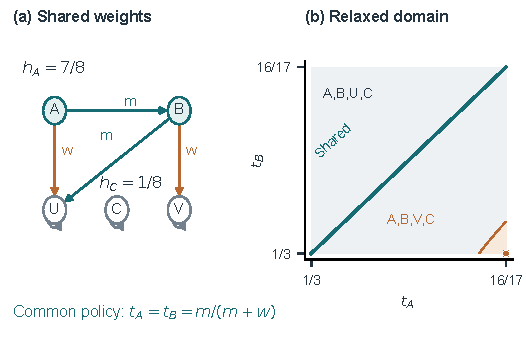
\includegraphics[width=\columnwidth]{../figures/domain_mechanism.pdf}
\caption{Shared dependence on an exact five-node graph. (a) Mention/weak edges are teal/orange; $U,V,C$ are absorbing, with $\alpha=1/2$. (b) Legal common weights lie on the diagonal and preserve top-4 $\{A,B,U,C\}$. Independent fractions admit a different set in the orange region. The marked corner is incompatible with one shared policy. Section~\ref{sec:constructed} gives exact formulas.}
\label{fig:mechanism}
\end{figure}

\subsection{Approximate responses and a posteriori error}
\label{sec:posterior}
Let $\widehat y,\widehat R_j$ be the full approximate vectors produced by the numerical solver. Only selected response coordinates must remain resident. Certified residual bounds satisfy
\begin{equation}
 \norm{A_0\widehat y-b}\leq\rho_y,\qquad
 \norm{A_0\widehat R_j+\alpha u_j}\leq\rho_j,
 \label{eq:residual}
\end{equation}
where $j$ indexes both groups. Construct $\widehat M$ using exact partition masses and source coordinates $\widehat H=E_S^T\widehat R$ of these \emph{same} full responses. Compile $\widehat D,\widehat C,\widehat F$ exactly from stored scalars. A source coordinate is untruncated, but its solver error remains covered by Eq.~\eqref{eq:residual}. Proposition~\ref{prop:degree} does not prove $\widehat D>0$; each certified cell establishes it separately.

Where $\widehat D>0$, let $\widehat x=\widehat y-\sum_j\widehat R_j\widehat F_j/\widehat D$. Its source relation implies $\widehat x_S=\operatorname{diag}(Z)\widehat C/\widehat D$. Consequently,
\begin{equation}
 \begin{aligned}
 (A_\theta\widehat x-b)\widehat D
 &= (A_0\widehat y-b)\widehat D\\
 &\quad-\sum_j(A_0\widehat R_j+\alpha u_j)\widehat F_j.
 \end{aligned}
 \label{eq:cancellation}
\end{equation}
The identity is exact for the stored approximate vectors. It cancels the source update without an additional inverse-norm factor for $\widehat M$. For a uniform induced-norm bound $\|A_\theta^{-1}\|_1\leq\kappa$,
\begin{equation}
 |x_i-\widehat x_i|\widehat D
 \leq\kappa\left(\rho_y\widehat D+\sum_j\rho_j|\widehat F_j|\right)
       +\epsilon\widehat D.
 \label{eq:posterior}
\end{equation}
The ideal stochastic model admits $\kappa=(1-\alpha)^{-1}$. An optional score allowance $\epsilon\geq0$ requires a separate justification; it is zero when all relevant error is already enclosed. Absolute amplitudes retain signed responses and sign changes across weight one. Neither $\widehat C\geq0$ nor $\widehat F\geq0$ is assumed.

\subsection{Contract for the stored graph}
\label{sec:raw}
The numerical target mathematically normalizes each selected source's stored raw mention/weak/self partition while keeping non-source raw columns fixed. Stored seed entries are interpreted exactly; exact unit-mass normalization would rescale all scores by one positive factor and preserve every top-$k$ membership. A stored column may sum to $1$ only up to rounding. Let $c_j>0$ be its exact sum, $\delta\geq\max_j|c_j-1|$, and $\bar c\geq\max_jc_j$. The canonical reference $P_*=P_{\rm raw}\operatorname{diag}(c)^{-1}$ is stochastic. The source core, responses, and partition masses in Eqs.~\eqref{eq:atoms}--\eqref{eq:posterior} are formed consistently against this reference. At a modified source, the common factor $1/c_s$ cancels in Eq.~\eqref{eq:policy}, giving the requested exact normalized source. Non-source background columns differ and require an allowance.

If $\rho_y^*,\rho_j^*$ bound residuals against the canonical reference, the a posteriori bound for the raw-background target uses
\begin{equation}
 \begin{aligned}
 \bar\rho_y&=\rho_y^*+\alpha\delta\norm{\widehat y},\\
 \bar\rho_j&=\rho_j^*+\alpha\delta\norm{\widehat R_j},\qquad
 \kappa=\frac1{1-\alpha\max(1,\bar c)}.
 \end{aligned}
 \label{eq:raw-contract}
\end{equation}
The denominator must be positive. The targets differ only on non-source columns, with induced $1$-norm at most $\delta$. Applying this perturbation to $\widehat x$ adds at most $\alpha\delta(\norm{\widehat y}\widehat D+\sum_j\norm{\widehat R_j}|\widehat F_j|)$ to its residual numerator. Equation~\eqref{eq:raw-contract} absorbs this term. Its resolvent multiplier follows from the raw target's column-norm bound $\max(1,\bar c)$.

The implementation uses exact dyadic source sums, right-hand-side conversion enclosures, signed sparse-matvec and norm-rounding bounds, and underflow allowances. Canonical residuals also enclose the correction from the raw backend. Actual-view witnesses cover materialized source-column conversion error. Polynomial controls are evaluated outward; the kernels require checked round-to-nearest binary64 arithmetic and gradual underflow without denormal-input flushing. A near-zero observed floating residual is not a substitute for these bounds. These shared premises support the mathematical target; a few point checks cannot establish the universal conclusion.

\section{Certifying Every Output Node}
\label{sec:certificate}
For response $j$, retain rows $I_j$ and a true omitted-coordinate bound $\tau_j\geq\max_{i\notin I_j}|\widehat R_j[i]|$. The candidate set $\mathcal C$ contains their union, all sources, and selected base candidates. Write $I(i)=\{j:i\in I_j\}$. Every source coordinate used in $\widehat M$ is retained consistently. A full-response layout can supply additional candidate coordinates: here $I_j$ denotes coordinates actually supplied, while a tail from a smaller retained set remains conservative. For outside nodes, let $\bar y=\max_{i\notin\mathcal C}\widehat y_i$.

On one cell, use the nonnegative tensor Bernstein basis of degree $(r,r)$, whose functions sum to one~\cite{sapo}. For control index $a$, let $\widehat D_a,\widehat F_{j,a}$ be the coefficients and $A_{j,a}=|\widehat F_{j,a}|$. The polynomial with controls $A_{j,a}$ bounds $|\widehat F_j|$ pointwise, including sign changes. Form
\begin{equation}
 \begin{aligned}
 B_{i,a}&=\widehat y_i\widehat D_a-
          \sum_{j\in I(i)}\widehat R_j[i]\widehat F_{j,a},\\
 T_{i,a}&=\sum_{j\notin I(i)}\tau_j A_{j,a},\\
 E_a&=\kappa\left(\rho_y\widehat D_a+\sum_j\rho_jA_{j,a}\right)
           +\epsilon\widehat D_a,\\
 O_a&=\bar y\widehat D_a+\sum_j\tau_jA_{j,a}.
 \end{aligned}
 \label{eq:controls}
\end{equation}
Here $T_{i,a}$ covers coordinate omission, $E_a$ covers a posteriori score error, and $O_a$ bounds every outside node's approximate numerator. The raw-input variant uses Eq.~\eqref{eq:raw-contract}.

\begin{theorem}[Whole-output domain certificate]
\label{thm:certificate}
Let $T\subseteq\mathcal C$ have size $k$. If every control has $\widehat D_a>0$ and
\begin{equation}
 \begin{aligned}
 \min_{i\in T}(B_{i,a}-T_{i,a})
 &>\max_{i\in\mathcal C\setminus T}(B_{i,a}+T_{i,a})+2E_a,\\
 \min_{i\in T}(B_{i,a}-T_{i,a})&>O_a+2E_a,
 \end{aligned}
 \label{eq:certificate}
\end{equation}
then $T$ is the strictly separated top-$k$ membership throughout the cell. Omit the second inequality if there are no outside nodes; an empty candidate-competitor maximum is $-\infty$.
\end{theorem}
\noindent\emph{Proof.}
Each full approximate candidate numerator lies between polynomials with controls $B_{i,a}-T_{i,a}$ and $B_{i,a}+T_{i,a}$, by the omitted-coordinate bounds and absolute $\widehat F_j$ envelope. Every outside approximate numerator is at most the polynomial with controls $O_a$, since $\widehat D>0$ and $\widehat y_i\leq\bar y$. The nonnegative Bernstein basis preserves each selected--competitor coefficient inequality at every policy. Equation~\eqref{eq:posterior} adds at most the polynomial with controls $E_a$ to either side. Positive $\widehat D$ permits division and establishes strict separation of the true scores.\hfill$\square$

The scan reduces node controls to selected minima and competitor maxima rather than enumerating all pairs. Several cutoffs share compilation and scanning, with separate conclusions. Failed sufficient tests may trigger subdivision. A complete cover by certified leaves establishes \stable; actual-view checks can establish \unstable; unresolved cuts remain \unknown. A negative approximate-determinant control or an insufficient gap is not an instability witness. A positive polynomial can also have an inconclusive coarse Bernstein enclosure, so subdivision refines the proof without changing the domain.

Figure~\ref{fig:output-certificate} separates the two dimensions of coverage. Source interactions remain coherent even when output coordinates are omitted. Candidate bounds and a tail bound cover the graph; Bernstein cells cover the policy rectangle. Both are required for a whole-domain top-$k$ conclusion.

\begin{figure}[t]
\centering
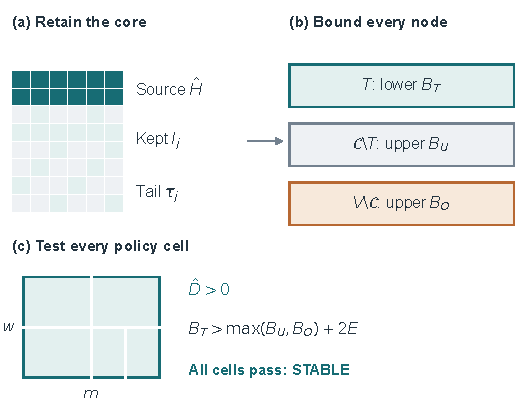
\includegraphics[width=\columnwidth]{../figures/domain_output_certificate.pdf}
\caption{Compressed whole-output certificate. (a) Source coordinates preserve the coherent core; retained rows and base preview form $\mathcal C$. (b) Bounds cover selected nodes, candidate competitors, and all outside nodes. (c) Every cell requires $\widehat D>0$ and the control inequalities in Eq.~\eqref{eq:certificate}, abbreviated as shown. The matrix and partition are schematic.}
\label{fig:output-certificate}
\end{figure}

\subsection{Two audits on one constructed graph}
\label{sec:constructed}
Use five nodes $A,B,U,V,C$, sources $A,B$, and $\alpha=1/2$. The base edges $A\to B$ and $B\to U$ are mention links; $A\to U$ and $B\to V$ are weak links, each of weight $1/2$. Nodes $U,V,C$ absorb. With $h=(7/8)e_A+(1/8)e_C$, $\Theta=[1,4]\times[.25,2]$, and $t=m/(m+w)$, scores are $x_A=7/16$, $x_B=7t/32$, $x_V=7t(1-t)/32$, $x_C=1/8$, and $x_U=7/16-7t/16+7t^2/32$. The top-4 set is always $\{A,B,U,C\}$. For example, $D=(m+w)^2/4$ gives $(x_C-x_V)D=(4m^2+mw+4w^2)/128>0$; the other three selected--$V$ gaps also have positive coefficients. A relaxation can let $A$ use $(4,.25)$ and $B$ use $(1,2)$, giving $x_V=7/51>1/8$ and $x_U=77/816<1/8$. This is not a shared-parameter witness (Fig.~\ref{fig:mechanism}). The polynomial test proves the parent box; lifting is initially \unknown\ and proves stability at depth two with three leaves. Both are sound.

The same graph shows why global corners can miss a change when $r\geq2$. With $h=.95e_A+.05e_C$ on $[.25,4]\times[.99,1.01]$, $x_V=.2375t(1-t)$ and $x_C=.05$. All four global corners have strict top-4 set $\{A,U,B,C\}$, but at $(1,1)$, $x_V=.059375>.05$, giving $\{A,U,B,V\}$. Both constructions were checked by exact rational full-system solutions. They illustrate logical issues rather than natural frequency. For $r=1$, cleared gaps are affine, so four strict corner certificates for one membership suffice throughout a rectangle; this supports the native control below.

\section{A Retained-State Domain Executor}
\label{sec:execution}
The implemented executor admits complete original source sets with $r\leq4$; it does not truncate larger requests. This is an implementation bound, while Proposition~\ref{prop:degree} applies to arbitrary finite $r$.
\subsection{Source interactions and output retention}
The directory is keyed by $(\text{group},\text{source})$. Registered original source sets define a stencil: each response retains the source rows needed to assemble complete cores for those combinations. It also retains its largest-magnitude output coordinates and a tail bound over all omissions. Registration does not populate responses for free; right-hand-side construction, graph solves, residual guards, tail extraction, and admission are charged. Unregistered combinations require their missing interactions to be admitted or a declared direct route.

For each question, a current-output preview $Q(h)$ contains the largest coordinates of $\widehat y$. Building or refining an atom retains its top-$L$ magnitudes, stencil rows, own source, and $Q(h)$. Values remain seed-independent; the preview only chooses where to retain them. A cache hit may carry an earlier question's preview. Each current family therefore adds its current $Q(h)$ to the candidates, without assuming those coordinates were retained by every hit. Missing entries remain covered by $T_{i,a}$. Preview selection and computing the maximum base score outside the candidates traverse the base vector and are charged.

This choice targets the current seed's output while preserving atomic reuse. Exploratory calibration considered no-preview retention and larger top-magnitude quotas before the primary was frozen. Accounting uses the actual union of stencil, preview, and top-$L$ rows, whose overlap determines retained bytes; admission reserves upper bounds for entries and working state not yet constructed. Complete-workload comparisons evaluate the resulting certificate and executor together.

\subsection{Admission, capacity, and precision}
A byte ledger admits resident atom values/indices, numerical metadata and interactions, plus family-private core/candidate/mask/proof state. Active atoms are pinned. Capacity pressure evicts unpinned least-recently-used atoms; a request whose working state cannot fit takes a recorded fallback. Full-response layouts borrow cached columns and stream candidate chunks rather than constructing an uncharged second $n\times q$ matrix, where $q\leq2r$. Sparse and scan layouts account for their allocated candidate matrices.

The retained-state budget is distinct from whole-process memory. Graphs, numerical backend state, current seed/base, and documented one-response generation and point-solve workspaces are separate. Control scans have explicit peak reservations. Payload reduction therefore need not imply proportional resident-set-size (RSS) reduction. Standalone measurements test that separate claim; paired experiments with several directories in one process cannot supply individual-method RSS.

The frozen primary uses fixed atom precision. An optional two-tier controller first tries coarse responses, then retries only \unknown\ cutoffs at fixed finer precision and retention. Certified stable cuts and verified unstable cuts are frozen. A cached atom is reusable if its actual generation tolerance and retained rows meet the requested tier. After the old family closes and releases pins, only inadequate needed keys are invalidated; unrelated atoms remain. Precision invalidations are counted separately from capacity evictions. If needed atoms already meet the final tier, an identical proof is not rerun under a new label. Complete controller cost includes both attempts, decisions, invalidations, releases, and solves.

\subsection{Shared compilation, scanning, and witnesses}
The small source core is compiled with exact rational arithmetic on stored scalars. A geometry-only monomial-to-Bernstein transform is reusable for the same box and degree; integer common-denominator dots avoid repeated fraction multiplication without approximating coefficients. Its cold preparation is charged to methods that use it. Child-cell transforms and compilation remain proof cost.

A chunked kernel computes node-control reductions for all cuts. The common accelerated backend first uses batched matrix products with coefficient-conversion radii, dot-product roundoff, and underflow bounds. Remaining \unknown\ cuts retry the outward-operation kernel. Both attempts are charged, the retry scans only unresolved cuts, and chunk storage is released before fallback. Applicable compressed, DensePruned, full-dense, and scan polynomial variants share this backend. It changes throughput rather than global parameter dependence or proof semantics.

The default schedule tries the certificate before expensive full-view checks. For a still-unresolved cut, actual-view solves at recorded in-domain policies may produce two strictly certified different memberships; only these establish \unstable. Each point solve includes source-column materialization, residual/conversion guards, and graph restoration. Native rank-one execution instead uses up to four adaptive-precision corner solves, shares them across cuts, and prepares neither responses nor a base vector. All calls and precision stages are recorded.

With $a=(r+1)^2$ tensor controls, a prepared scan costs $O(|\mathcal C|qa)$ per visited cell and uses chunk-bounded control workspace. Exact compilation depends on $r$ and coefficient bit lengths. Base traversal and response preparation still depend on graph size and sparsity. Reuse saves preparation only when the ordered trace revisits useful keys; neither high hit rate nor high certificate rate alone establishes a total-time advantage.

\section{Evaluation Design and Evidence}
\label{sec:evaluation}
We separate the universal operator from its retained representation. The first comparison asks whether preserving common dependence helps against strong regional controls under the same output contract. The second asks what compressed retention gains or loses against the same polynomial proof with full responses. Section~\ref{sec:domain-results} reports the complete fixed workloads and distinguishes separately scheduled cohorts.

\subsection{Inputs, queries, and frozen configuration}
The primary graphs pool public development contexts from HotpotQA~\cite{hotpot} and MuSiQue-Ans~\cite{musique}, rather than making a tiny graph per question. Passage identity includes title, exact text, and handling of duplicate occurrences; title alone does not merge distinct passages. The HotpotQA pool has 66,635 nodes and 2,352,679 stored transitions from all 7,405 development questions, with the first 1,000 original questions timed in fixed order. MuSiQue has 21,100 nodes and 625,618 transitions and uses all 2,417 original development questions. The Hotpot subset is a declared execution workload, not full development-set evaluation. A question is the sampling unit; its cuts, domain cells, and probed policies are not independent question samples.

Both use lexical BM25 seeding, exact title-mention links, sparse rare-term associations, and $\alpha=.5$. Seeding normalizes the top 32 BM25 scores, with a uniform fallback if all scores vanish. The original source extractor orders question title matches by decreasing title length and then node identifier, taking at most four; without a match it takes the top two BM25 nodes. It retains chosen columns changed by its fixed $(3,.5)$ selection probe. This extractor imposes $r\leq4$; execution uses each original source array in full. The audit box is $[1,4]\times[.25,2]$, with $k\in\{2,5,10\}$. Question/context fields determine inputs; support labels and answers do not select sources, weights, tolerances, or retention. Execution is evaluated against this declared policy, rather than credited with quality gains from changing it.

The complete primary plans register 8,477/8,098 directed source pairs (HotpotQA/MuSiQue), compared with 3,374,569/5,008,644 pairs in their complete source universes. The stencils use only submitted source identifiers. Multi-source questions constitute 901/1,000 and 1,657/2,417 requests, respectively.

The primary was frozen after exploratory calibration and before complete evaluation: $L=512$, preview size $128$, atom tolerance $10^{-6}$, base tolerance $10^{-10}$, maximum polynomial depth two, the common dot-plus-outward backend, and 16\,MiB retained-state admission budget. The protocol specifies three ordered cold-directory blocks per dataset, paired inputs, original question identifiers, source hashes, and deterministic method orders. Calibration prefixes and two-query checks select or validate the setup. Their exploratory measurements are separate from complete-workload summaries; selected calibration cases below serve as mechanism illustrations.

Experiments use an AMD Ryzen 9 9950X (16 cores, 32 logical CPUs), 32\,GiB installed memory, Windows 11 Pro, Python 3.10.6, NumPy 2.2.6, SciPy 1.15.3, and a native PRPACK backend~\cite{prpack}. Our adapter exposes unnormalized signed right-hand-side solves and fixed-support numerical refresh while reusing its SCC structure. Every timed producer is pinned to one logical CPU with one BLAS thread and the same recorded above-normal process priority. The three blocks run on a shared interactive host. We retain every block and use paired comparisons and descriptive ranges to expose timing variability.

The graph builder adds raw self weight $0.5$ at every node before column normalization. An exact stored-partition audit finds no zero-self source among the 1,837/2,238 unique modified HotpotQA/MuSiQue sources. Their normalized self masses range from $3.002\times10^{-6}$ to $0.1163$ and $1.028\times10^{-5}$ to $0.3685$, respectively. Disjoint-group support checks and source-direction ranks identify genuinely two-dimensional policy changes in 980/1,000 and 2,395/2,417 original requests. The remaining 20/22 are one-dimensional special cases; the workload is not globally a ratio-only intervention.

\subsection{Strong controls and mechanism ablations}
\begin{table}[t]
\centering\small
\caption{Method roles under a common domain/output contract. Both DensePruned precisions and the atom-free single-source route remain strong controls.}
\label{tab:methods}
\begin{tabular}{@{}p{.26\columnwidth}p{.66\columnwidth}@{}}
\toprule
Method & Representation or logical difference\\
\midrule
Sparse primary & Shared polynomial proof; compressed atoms, source stencil, current-base preview.\\
Poly DensePruned & Same polynomial/candidates/tails; full responses supply more candidate entries. Atom tolerances $10^{-4}$ and $10^{-6}$.\\
Source-wise LiftDP & Pruned full-response layout, independent source policies, depth-four refinement.\\
Source-wise LiftSparse & Same compressed atoms and preview as primary; independent source policies, depth four.\\
Native + LiftDP & Atom-free four-corner route for $r=1$; LiftDP for $r\geq2$.\\
Full / Scan & All-row output scan with dense / compressed responses.\\
Interval / NoCore & Remove coefficient dependence / accurate source interactions; re-establish the altered residual contract.\\
\bottomrule
\end{tabular}
\end{table}

DensePruned shares the core, polynomials, candidate construction, a posteriori error, and outside-node proof. Full columns provide additional exact candidate entries. It is both a physical variant and the strongest own-layout control for compression (Table~\ref{tab:methods}). Both declared precisions remain visible; no per-question best-method oracle is formed.

The regional baseline implements source-wise lifting following parameter relaxation~\cite{lifting}. A normalized source at any rectangle point lies in the convex hull of its corner distributions. Bilinear interpolation expresses its affine numerator and positive affine normalizer with the same nonnegative corner weights. Multiplying each weight by its corner normalizer and dividing by the interpolated normalizer gives a convex combination of corner columns. Holding the other columns fixed, each true score gap is linear-fractional in one source column with a positive denominator; its extrema lie at corner columns. Applying this successively justifies the corner policies of the independent-source relaxation. This relaxation is sound, although it can lose one common $(m,w)$. The implementation shares preparation and candidate scanning, uses small source systems, and permits depth four versus the primary's two. This stronger declared schedule is charged in full. A further layout-matched lifting control uses the same compressed retention and preview as the primary, separating parameter dependence from full-column cache cost; its separately frozen cohort must be identified with its results. Relaxed policies never serve as actual witnesses.

The lifting implementation deduplicates identical normalized corner columns, enumerates their independent source combinations, and solves each small core exactly. For its response coefficients $\beta_j$, the score allowance is $\kappa(\rho_y+\sum_j\rho_j|\beta_j|)+\epsilon$, plus retained-coordinate tails and outward conversion/dot guards. Selected lower bounds must exceed candidate and outside upper bounds for every relaxed policy. An unresolved cell bisects its longest weight interval; depth four is the limit. A cutoff is stable only when both children succeed; singular cores or terminal unseparated gaps return \unknown. Actual-view witness search is a separate shared execution stage. This specifies the baseline's error handling, subdivision axis, and stopping rule without treating a mixed-source counterpolicy as instability.

For $r=1$, affine cleared gaps make strict common corner membership sufficient throughout the rectangle. The native hybrid uses this special case directly. Adaptive corner tolerances stop once all requested cuts are established; two real strict different sets can stop instability detection early. For $r\geq2$, the same strong lifting path applies. This control avoids forcing atomic preparation when direct corners suffice.

Mechanism studies keep the graph, seed, domain and output contract fixed. Independent coefficient intervals enclose each $F_j/D$ separately on a cell, then reconstruct score intervals with the same residual and tail premises, discarding common polynomial dependence. NoCore zero-fills omitted response coordinates, builds its source core from that truncated model, and recomputes the model's full residual bound. It jointly changes retained source interactions and posterior error, exposing the value of preserving their coherent full-response contract. Scan retains sparse atoms but scans every output row. The fixed two-tier \unknown-only controller remains optional. A separate capacity study disables actual-view witness search equally for all methods at 1, 4 and 16\,MiB and measures questions with all three cutoffs certified \stable. The full-operator comparisons retain witness search and report complete three-valued audit resolution.

\subsection{Cost, coverage, and memory accounting}
Primary time is complete active-operator cost over every query in the ordered trace. It charges method-owned setup and applicable common startup, base computation or explicit reuse, source/right-hand-side construction, misses, residual guards, preview selection, admission/eviction, exact compilation, all scans/subdivisions, witnesses, refinement, and release. Graph loading, imports, serialization, and independent auditing are identified separately and excluded symmetrically. A method needing neither base nor Bernstein transform does not pay those stages. There is no free atom bank, post-hoc warm directory, or uncharged final precise pass.

All \unknown\ requests remain in time denominators. We report per-cut \stable, verified \unstable, and \unknown\ counts, plus questions with all three cuts resolved. All-question active-query $p95$ includes misses/refinement and is not multi-user service latency. Repeated blocks expose timing variability. Different resolved populations are time/coverage tradeoffs, not equal-completion speedups. Source-count strata distinguish native $r=1$ from coupled $r\geq2$. Counters record solves, hits, capacity evictions, precision invalidations, visited cells, and actual point checks to expose causes.

The ledger reports resident payload and peak admission state including family-private allocations. Separate fresh-process Sparse, fine DensePruned, and compressed lifting runs measure operating-system peak working set and producer wall time; paired peaks describe the combined process. Graph/backend and documented generation workspaces remain visible alongside retained-state accounting.

\subsection{Complete-workload operator comparison}
\label{sec:domain-results}
Table~\ref{tab:domain-main} reports the fixed workloads, including startup, method-owned setup, all query stages, and unresolved requests. Times and p95 values are medians of three complete blocks; coverage requires every requested cutoff resolved. All block values are retained in the artifact.
\begin{table*}[t]\centering\small
\caption{Complete policy-domain workloads at 16 MiB retained-state budget. Total seconds and p95 milliseconds are complete-block medians; resolved coverage requires all three cutoffs. DensePruned shares ViewRank\textquotesingle s polynomial certificate. The separated bottom panel is an independent paired cohort with the same compressed representation for both certificates. Compare costs within a panel; absolute times are not pooled across cohorts.}
\label{tab:domain-main}
\begin{tabular}{lrrrrrr}\toprule
& \multicolumn{3}{c}{HotpotQA, 1,000 questions}&\multicolumn{3}{c}{MuSiQue, 2,417 questions}\\
Method & Total (s)&Resolved (\%)&p95 (ms)&Total (s)&Resolved (\%)&p95 (ms)\\\midrule
ViewRank--Sparse & 116.81 & 99.70 & 250.4 & 108.58 & 98.97 & 165.4\\
ViewRank--DensePruned ($10^{-4}$) & 116.46 & 99.30 & 213.9 & 98.03 & 98.47 & 125.5\\
ViewRank--DensePruned ($10^{-6}$) & 136.16 & 99.80 & 229.0 & 103.77 & 99.01 & 127.3\\
Source lifting, full responses & 200.12 & 99.20 & 371.3 & 311.10 & 98.10 & 481.8\\
Native rank-one + source lifting & 215.77 & 99.20 & 369.1 & 340.62 & 98.10 & 479.2\\
\midrule
\multicolumn{7}{l}{\emph{Separate paired cohort A: same compressed representation}}\\
ViewRank--Sparse (paired A) & 129.00 & 99.70 & 276.4 & 113.24 & 98.97 & 178.8\\
SourceLift, compressed (paired A) & 198.00 & 99.20 & 379.7 & 331.59 & 98.06 & 533.2\\
\bottomrule\end{tabular}\end{table*}
The strongest layout-matched comparison is cohort A. Both methods use sparse $L=512$ retention, 128 current-base preview coordinates, and atom tolerance $10^{-6}$; SourceLift receives subdivision depth four. ViewRank--Sparse lowers complete-workload cost in every paired block: 34.7--35.3\% on HotpotQA and 65.9--66.0\% on MuSiQue. All original requests and unresolved outcomes remain included.
Complete-audit counts are 997 versus 992 on HotpotQA and 2392 versus 2370 on MuSiQue, identical across repetitions. Median all-question p95 values are 276.4 versus 379.7 ms and 178.8 versus 533.2 ms, respectively. The shared-domain certificate therefore improves complete cost, resolution and tail latency after matching compressed retention.
The original main cohort also compares full-response source lifting: the primary reduces complete cost by 40.9--41.6\% on HotpotQA and 64.8--65.1\% on MuSiQue. The atom-free rank-one hybrid remains visible alongside it.
The same certificate supports complementary physical layouts. Sparse retention reduces HotpotQA total cost by 14.2\% relative to same-tolerance DensePruned, while DensePruned gives lower total cost on MuSiQue. The fine full-response layout resolves one additional question on each dataset.
\begin{figure}[t]\centering
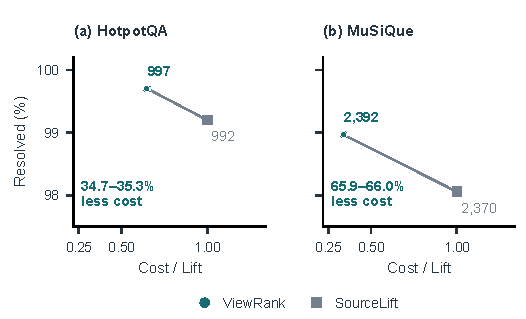
\includegraphics[width=\columnwidth]{../figures/domain_performance.pdf}
\caption{Complete cost and resolution in layout-matched cohort A at 16\,MiB: 1,000/2,417 HotpotQA/MuSiQue questions. Cost is divided by paired compressed SourceLift; all three blocks are plotted and can overlap. Lines join median operating points. Counts require all three cutoffs resolved (\stable\ or verified \unstable); the labeled vertical range magnifies the small coverage differences. All requests, including \unknown, remain charged.}
\label{fig:domain-performance}
\end{figure}
Figure~\ref{fig:domain-performance} places the strongest layout-matched comparison in the cost--resolution plane: ViewRank moves toward lower complete cost and more resolved audits on both workloads. Figure~\ref{fig:domain-coupling} locates the largest active-cost gains in the coupled-source work addressed by the compiler. Table~\ref{tab:domain-main} separately retains the competitive DensePruned layouts and the original full-response controls.

\begin{figure}[t]\centering
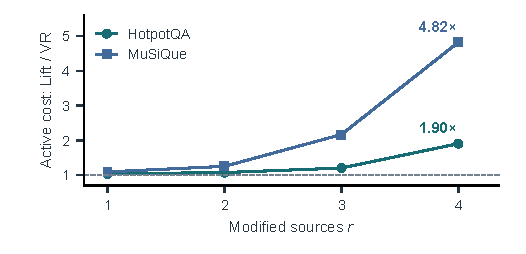
\includegraphics[width=\columnwidth]{../figures/domain_coupling.pdf}
\caption{Source-count strata in cohort A. Lines join medians of three paired ratios of summed active cost; dots retain every block. Every stratum includes \unknown\ requests. Startup/setup are excluded here. Repeated blocks are descriptive, not confidence intervals.}
\label{fig:domain-coupling}\end{figure}

\IfFileExists{generated/domain_source_count.tex}{The $r=1,2,3,4$ strata in Fig.~\ref{fig:domain-coupling} contain 99/232/220/449 original HotpotQA questions and 760/797/253/607 MuSiQue questions. Median SourceLift/ViewRank active-cost ratios are 1.03/1.07/1.20/1.90 and 1.09/1.25/2.17/4.82, respectively. Every stratum and unresolved request remains included; the artifact retains all paired values and counts.
}{}
% Remaining component controls, budgets and fresh-process memory come from their own complete cohorts.
\IfFileExists{generated/domain_supplement_results.tex}{\subsection{Matched mechanism controls}
Table~\ref{tab:domain-ablation} gives a separately scheduled paired block of each complete workload. All methods use the same original questions, policy domain, cutoffs, and 16\,MiB budget. Fixed-precision controls use the primary\textquotesingle s $10^{-6}$ response tolerance. Total costs include every unresolved request; the controller includes both tiers and all retries.
\begin{table}[t]\centering\footnotesize\setlength{\tabcolsep}{2.5pt}
\caption{Matched complete-workload controls, one block per graph. Resolved coverage requires all three cutoffs of a question.}
\label{tab:domain-ablation}
\begin{tabular}{lrrrr}\toprule
&\multicolumn{2}{c}{HotpotQA}&\multicolumn{2}{c}{MuSiQue}\\
Method&Time (s)&Done (\%)&Time (s)&Done (\%)\\\midrule
ViewRank--Sparse & 149.02 & 99.70 & 169.45 & 98.97\\
NoCore & 309.31 & 22.20 & 476.09 & 16.84\\
All-row Scan & 761.84 & 99.80 & 779.80 & 98.97\\
Independent intervals & 143.02 & 46.70 & 140.28 & 52.42\\
Two-tier controller & 138.31 & 99.80 & 199.21 & 99.01\\
\bottomrule\end{tabular}\end{table}
\begin{figure}[t]\centering
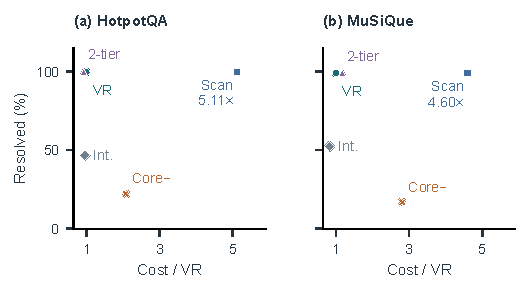
\includegraphics[width=\columnwidth]{../figures/domain_controls.pdf}
\caption{Matched component controls, one complete block per graph. VR: ViewRank; Core$-$: NoCore; Scan: all-row scan; Int.: independent intervals; 2-tier: optional controller. Cost includes all original requests and is normalized to paired VR. Read resolution jointly; Table~\ref{tab:domain-ablation} retains absolute values.}
\label{fig:domain-controls}\end{figure}
Figure~\ref{fig:domain-controls} makes the component effects visible jointly: a cheaper but unresolved workload is distinct from a complete-cost improvement at comparable or better resolution.
All-row Scan costs 5.11$\times$/4.60$\times$ VR on HotpotQA/MuSiQue with nearly identical resolution (Table~\ref{tab:domain-ablation}). NoCore changes both source coherence and its recertified posterior allowance, raising total cost while reducing completion to 222/407 questions. Independent intervals cost 4.0\%/17.2\% less but resolve only 467/1267 questions, so their saving is a cost--coverage tradeoff. The optional controller is 7.2\% faster on HotpotQA and 17.6\% slower on MuSiQue; its p95 rises to 404.3/338.7\,ms from 305.9/234.3\,ms. Fixed fine precision remains the primary.

\subsection{Certificate capacity and process memory}
Figure~\ref{fig:domain-budget} reports separate witness-free certificate-capacity runs: one paired block per graph at each budget. Success requires all three cutoffs STABLE for an original question. Tables~\ref{tab:domain-main} and~\ref{tab:domain-ablation} instead report complete three-valued audit resolution.
\begin{figure}[t]\centering
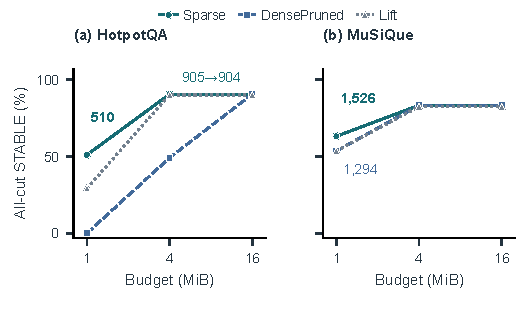
\includegraphics[width=\columnwidth]{../figures/domain_budget.pdf}
\caption{Certificate capacity at 1/4/16\,MiB: Sparse and DensePruned use the same polynomial proof; Lift uses compressed source lifting. Counts label selected points. Every original question remains in the denominator; success requires all three cutoffs \stable. Witness search is uniformly off. One block per setting; admitted numerical state is distinct from process memory.}
\label{fig:domain-budget}\end{figure}
At 1\,MiB, Sparse certifies all cutoffs for 510/1000 versus 0 for DensePruned and 293 for sparse lifting on HotpotQA; the corresponding MuSiQue counts are 1526/2417 versus 1294 for DensePruned and 1296 for sparse lifting.
At 4\,MiB, compressed retention certifies exactly the same 905 HotpotQA and 2014 MuSiQue original questions as fine DensePruned at 16\,MiB. Independent comparison confirms identical question sets and memberships at every cutoff. These are the measured configurations in Fig.~\ref{fig:domain-budget}. The Sparse HotpotQA counts are 905 at 4\,MiB and 904 at 16\,MiB; preview rows depend on cache-miss history and need not be nested across budgets. All attempted work remains charged.
\begin{table}[t]\centering\footnotesize\setlength{\tabcolsep}{2.5pt}
\caption{Fresh single-method processes, one complete run per graph at 16\,MiB with fine responses and no audit serialization. Wall is recorded producer time (seconds); peak is the cumulative process peak working set (MiB) read at block end, including the graph and backend.}
\label{tab:domain-memory}
\begin{tabular}{lrrrr}\toprule
&\multicolumn{2}{c}{HotpotQA}&\multicolumn{2}{c}{MuSiQue}\\
Method&Wall&Peak&Wall&Peak\\\midrule
ViewRank--Sparse & 140.17 & 368.8 & 117.73 & 170.1\\
DensePruned & 162.54 & 424.2 & 110.23 & 179.6\\
SourceLift, compressed & 199.81 & 356.9 & 353.26 & 166.9\\
\bottomrule\end{tabular}\end{table}
Table~\ref{tab:domain-memory} uses fresh single-method processes without audit serialization. Wall spans source freezing through execution, excluding final-summary serialization; cumulative OS working-set peaks include the graph/backend and generation scratch as well as admitted state.
}{}

% Displayed certificate lower bounds round down; upper bounds round up.
\subsection{Shared dependence on natural queries}
The complete calibration prefixes contain three question--cutoff pairs,
out of 600, for which the shared-parameter certificate proves stability
while fine DensePruned source lifting remains unresolved at depth four.
We select one case per graph by decreasing source count and then increasing
original question index (Table~\ref{tab:natural-dependence}).
Both methods cold-miss all atoms at the same $10^{-6}$ tolerance in these
cases. The independently verified mixed-source policies below expose a concrete
gap introduced by independent-source relaxation.

\begin{table}[t]\centering\small
\caption{Selected natural mechanism cases. The polynomial certificate proves
the complete rectangle in one cell. The last column bounds a selected-minus-
outside score gap for an independently verified mixed-source corner policy
inside an unresolved lifting leaf.}
\label{tab:natural-dependence}
\begin{tabular}{lrrrr}\toprule
Question & $r$ & $k$ & Lift cells & Gap upper bound\\\midrule
HotpotQA 68 & 4 & 10 & 9 & $-2.041\!\times\!10^{-8}$\\
MuSiQue 66 & 2 & 5 & 25 & $-8.568\!\times\!10^{-6}$\\
\bottomrule\end{tabular}
\end{table}

For HotpotQA 68, a terminal cell
$[1,7/4]\times[25/16,2]$ admits the source-specific assignments
$(1,2),(7/4,25/16),(1,25/16),(1,25/16)$.
Exact reconstruction of the saved small core and retained boundary rows,
including the a posteriori allowance, proves that outside node 18429
outranks selected node 678. For MuSiQue 66, the assignments
$(7/4,1/4),(1,11/16)$ inside
$[1,7/4]\times[1/4,11/16]$ make outside node 1087 outrank selected node 1091.
Both pair comparisons use fully retained rows. Independent exact
Leibniz/Cramer calculations reproduce the coefficients and guarded negative
bounds. These mixed-source policies are permitted by the relaxation but
excluded by the shared weights, whose entire rectangle is certified stable.
The cases demonstrate a concrete source of tightening; complete-workload
costs and coverage quantify its aggregate value.

\subsection{Shared-parameter verifier and operating boundaries}
The new studies address verifier choice and operating conditions separately from the complete three-block primary workloads. All prefixes, source arrays and methods are fixed before each study; every requested cutoff remains in its denominator.
\begin{table}[t]\centering\footnotesize\setlength{\tabcolsep}{3pt}
\caption{Shared-core verifier comparison, first 20 questions per graph, all 60 cutoffs. Entries are seconds / STABLE cuts. Both consume identical retained rows, tails and upward-rounded residual/resolvent bounds. SMT has a 5\,s solver limit per cutoff; all encoding time is included. One block; graph preparation and the common compiler are excluded.}
\label{tab:shared-smt}
\begin{tabular}{lrr}\toprule Graph & Bernstein & Shared SMT\\\midrule
HotpotQA & 0.683/57 & 327.87/0\\
MuSiQue & 0.118/57 & 156.19/33\\
\bottomrule\end{tabular}\end{table}
The solution-function comparator follows the shared-parameter SMT route of Junges et al.~\cite{junges2024}, implemented here with Z3 QF\_NRA rather than the PROPhESY tool. It asks whether any in-domain policy has nonpositive approximate determinant or violates a guarded selected--competitor gap, including all outside nodes through the same tails. UNSAT certifies stability; SAT only refutes this sufficient test and is not an actual instability witness. The three MuSiQue SAT cases remain UNKNOWN; the other unproved SMT cuts time out. Table~\ref{tab:shared-smt} isolates verification on the same source core; it is not an end-to-end or solver-workspace-budget-matched comparison. The SMT baseline passes an independent exact three-node positive/negative membership check.
The encoding names $D$ and all $2r$ amplitudes $F_j$, constrained to their exact monomial polynomials. Let $N_i,T_i,E,O$ be the pointwise forms of Eq.~\eqref{eq:controls}, using $|F_j|$ instead of coefficient envelopes, with $\epsilon=0$ in both verifiers. Put $L_i=N_i-T_i-2E$ and $U_i=N_i+T_i$. Within the box and polynomial equalities it checks satisfiability of
\begin{equation}
\begin{aligned}
 &(D\leq0)\ \lor\ \bigvee_{i\in T}(L_i\leq O)\\
 &\quad\lor\ \exists z:\left(\bigvee_{i\in T}L_i\leq z\right)
              \land\left(\bigvee_{j\in\mathcal C\setminus T}U_j\geq z\right).
\end{aligned}
\label{eq:smt-encoding}
\end{equation}
The threshold $z$ avoids enumerating $k(|\mathcal C|-k)$ pairs. There are $1+2r$ polynomial equalities, four box inequalities, $|\mathcal C|$ threshold inequalities and $k$ outside-gap inequalities, plus the determinant and amplitude sign tests. The 120 encodings have 597--1,967 candidates and 6,035--23,701 unique Z3 expression nodes. Each cutoff shares its named expressions internally but builds a fresh solver; there is no cross-cutoff encoding reuse. We use Z3 5.3.3 (package 5.3.3.0), \texttt{SolverFor(QF\_NRA)}, seed zero, and the logic-specific default strategy without a custom tactic. HotpotQA encoding/solve totals are 18.76/309.10\,s; MuSiQue totals are 8.11/148.08\,s. All cutoff times, constraint counts and an SMT-LIB export accompany the artifact.

\begin{table}[t]\centering\footnotesize\setlength{\tabcolsep}{2pt}
\caption{Propagation boundary on fixed first-100 prefixes, one complete paired block at each setting. Cells: complete seconds / all-cut resolved questions / UNKNOWN cutoffs. VR: Sparse; DP: fine DensePruned; Lift: compressed SourceLift. Every original prefix request remains charged.}
\label{tab:alpha-boundary}
\begin{tabular}{lrrr}\toprule Graph, $\alpha$ & VR & DP & Lift\\\midrule
Hot, 0.50 & 16.1/99/1 & 16.8/99/1 & 22.3/97/3\\
Hot, 0.85 & 38.1/99/1 & 38.8/99/1 & 49.7/99/1\\
Hot, 0.95 & 95.4/100/0 & 99.0/100/0 & 98.4/100/0\\
Mu, 0.50 & 5.2/98/2 & 5.0/98/2 & 9.4/97/3\\
Mu, 0.85 & 10.4/99/1 & 10.4/99/1 & 12.9/99/1\\
Mu, 0.95 & 23.3/100/0 & 23.0/100/0 & 29.0/100/0\\
\bottomrule\end{tabular}\end{table}
At $\alpha=.95$, both primary prefixes resolve all 100 requests. HotpotQA is near parity with compressed lifting (3.1\% lower cost in this block); MuSiQue retains 19.8\% lower cost. Figure~\ref{fig:boundary-stages} separates the increased graph-response work from audit work. These are controlled operating points, not new independent questions or three-block confidence intervals.
\begin{figure}[t]\centering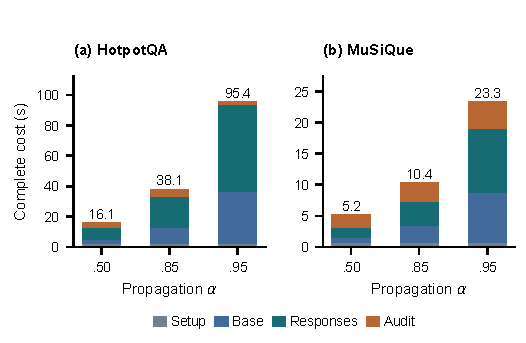
\includegraphics[width=\columnwidth]{../figures/domain_boundary_v3.pdf}
\caption{Primary complete-cost stages for Table~\ref{tab:alpha-boundary}. Base includes seed construction; Audit includes certification, actual witnesses and release; Setup includes charged startup and method setup. One complete block per setting.}
\label{fig:boundary-stages}\end{figure}
\begin{table}[t]\centering\footnotesize\setlength{\tabcolsep}{2pt}
\caption{Additional graph contexts and controlled Amazon probes; same cell format as Table~\ref{tab:alpha-boundary}. Small lexical pools use 100 queries and $\alpha=.5$. Amazon has 334,863 nodes, $\alpha=.85$, and all eight pre-existing $r=4$ seed/source requests. $+$self adds raw self weight .5 before normalization. One complete paired block; 16\,MiB admission budget.}
\label{tab:graph-boundary}
\begin{tabular}{lrrr}\toprule Graph (nodes) & VR & DP & Lift\\\midrule
Hot (9,769) & 3.9/100/0 & 3.2/100/0 & 12.0/99/1\\
Mu (12,493) & 3.3/99/1 & 3.1/99/1 & 6.4/98/2\\
Amazon & 23.7/8/0 & 40.8/3/8 & 38.0/8/0\\
Amazon +self & 22.8/8/0 & 40.4/3/8 & 38.1/8/0\\
\bottomrule\end{tabular}\end{table}
The smaller natural context pools retain their declared graph-dependent seeds/sources, so the comparison with the full pools changes graph context as well as size. Amazon uses a fixed hash-based neighbor grouping, not semantic mention links. Its zero-self original is a ratio-only control; the added-self variant exercises two policy directions. Both preserve the complete selected source arrays. The eight original $r=16$ requests are outside the current implementation\textquotesingle s $r\le4$ admission contract and receive no performance claim. Sparse resolves 8/8 in both probes, versus 3/8 for DP, and reduces complete cost against compressed lifting by 37.7\%/40.0\%. These limited probes extend execution evidence beyond the lexical topology without establishing application accuracy.
Across these ten complete cohorts, the primary's admitted numerical-state peaks span 2.98--5.79 MiB. Fresh cohort process peaks span 102.0--373.0 MiB and include all three paired method directories plus graph/backend state; they are not individual-method RSS values. Exact stage and memory records accompany the tables.

Table~\ref{tab:tristates} separates stability, verified sensitivity and unresolved cuts. At $\alpha=.95$, resolving all 100 primary queries includes 1/27 unstable HotpotQA/MuSiQue cuts. Each Amazon DP probe returns 0/16/8: its eight dense response vectors alone require 21,431,232 bytes, exceeding 16\,MiB; this route needs no stencil registration. Actual-policy searches then prove 16 cuts unstable, leaving eight unresolved. Other cohorts' unresolved leaves report insufficient candidate/relaxed-gap separation at the fixed depth. The artifact preserves every reason and witness-search count.
\input{../results/submission_details_v4/tristates.tex}

Amazon uses SNAP's \texttt{com-amazon.ungraph}~\cite{snapamazon}: 334,863 nodes, 925,872 undirected edges, expanded to 1,851,744 directed entries and column-normalized. Sorted original IDs define coordinates. The degree-ordered top-128 directory (ties by ID) supplies its first eight one-hot seeds. Each original source set takes four eligible nodes ordered by decreasing base PPR, degree, then increasing ID. A stable SHA256 ordering of source/destination pairs selects half each source's neighbors for the first group. The artifact gives the exact hash recipe, raw-file SHA256, all seeds/source arrays and self-loop construction.

\subsection{Reproducibility access}
The public artifact at \url{https://github.com/fuxiaoji/ViewRank} maps tables to fixed inputs, configurations, complete ledgers and commands. Release assets include graphs, proof states, source snapshots and all 120 SMT cutoff records. One entrypoint checks hashes, rebuilds table data and replays a certificate; numerical reruns write separate outputs.

\subsection{Verification scope and policy sensitivity}
The implementation passes 264 tests. Independent premise audits cover 52 representative complete responses, 2,190,040 residual coordinates, 412 exact sparse dot products, and exact column-mass sums over all 2,978,297 transition values in 87,735 columns. They check source partitions, RHS conversion, retained/source coordinates, norms and omitted tails; the 52-response audit is not a re-solve of every generated response.

Whole-domain scalar proof replay covers all 9,674 distinct primary \stable\ question--cutoff targets: 9,617 proof executions plus 57 within-block exact-identity reuses. Repeated blocks yield 29,022 covered stable instances, with no fast/scalar disagreements. The scalar checker shares the source-local formulation, so this coverage is distinct from the independent numerical-premise audit. Two additional stable targets from other layouts are proved using fresh signed responses, independent residual/tail checks, and a scalar certificate over the parent box; primary unresolved outputs remain unchanged. All 16 original supplementary cohorts pass ledger/output checks: 199,786 repeated stable instances match proved memberships and 7,686 unstable instances match verified actual-view records. Repeats are not additional questions.

The 549 distinct primary \unstable\ cutoffs occur in 475 of 3,417 original questions (13.9\%). Thus the observed policy sensitivity extends beyond the displayed example. Independent cold solves at 1,133 query--parameter points verify the actual changed memberships and strict gaps; the remaining 28 cutoffs stay \unknown. Stable outputs permit membership reuse over the specified range; unstable outputs supply concrete replacements for inspection. This interpretation concerns the declared ranking policy, rather than downstream answer accuracy.


\section{Related Work and Positioning}
\label{sec:related}
Ranking sensitivity has direct database foundations. Soliman et al.~\cite{uncertainranking} study uncertain scoring weights, top-$K$ semantics, and sensitivity to preference refinement. Asudeh et al.~\cite{stablerankings} study stable rankings in acceptable weight regions, including ordered and unordered top-$k$. Their attribute-score setting yields geometric ranking regions. Our normalized graph propagation produces rational scores and adds a numerical execution contract: approximate responses and omitted output coordinates must remain covered throughout the region.

Bojchevski and G\"unnemann~\cite{graphcert} connect PageRank and MDPs to certify output robustness under graph perturbations, including budgeted structural changes. Our shared continuous weights, local intervention set, and top-$k$ membership audit differ from their perturbation sets and classification setting. Graph-output certification itself is an established objective.

Junges et al.~\cite{junges2024} give shared-parameter SMT region verification, using original equations or solution functions, implemented in PROPhESY. Thus parameter dependence can be preserved by existing verification routes. ViewRank specializes the representation to a source-local affine core and couples its solution functions to posterior residual and output-tail bounds. A shared-core verifier comparison can isolate this latter contribution from the loss of dependence in source-wise lifting.

PPR solving and edge-weight personalization supply the numerical foundation. Maehara et al.~\cite{maehara} exploit graph structure; EdgePPR~\cite{edgeppr} uses model reduction for edge weights. Its sampled reduced subspace approximates point-policy score maps and includes Petrov--Galerkin approximation error theory. Here the exact-response source reduction is an algebraic identity; approximate graph responses enter with explicit residual and omitted-output bounds. OSP~\cite{osp} propagates offsets after graph changes, and EvePPR~\cite{eveppr} handles changes to graph and personalization. ViewRank builds on local elimination and reusable responses to establish universal membership over shared normalized weights, adding a posteriori error and all-output omission bounds.

Symbolic parametric Markov-chain analysis computes rational quantitative functions. Hutschenreiter et al.~\cite{parametric} study parametric systems and fraction-free elimination, including rational representations and complexity. Our compiler first reduces the graph query to modified sources, so local dimension governs degree. It links these comparisons to approximate numerical responses and the requested output boundary, specializing rational analysis to a source-local graph operator.

Quatmann et al.~\cite{lifting} replace parametric transitions by nondeterministic extremal choices to obtain sound, refinable bounds. Our source-wise control follows that relaxation principle, with a convex-hull argument for normalized columns. The comparison exposes the value of preserving shared dependence: the polynomial representation excludes incompatible source choices directly, while lifting can recover precision by subdivision.

Bernstein enclosure and subdivision are established in polynomial verification; Sapo~\cite{sapo} uses them for polynomial dynamics and parameter synthesis. ViewRank connects source-local score numerators to absolute response amplitudes, residuals, and omitted-coordinate tails in one sufficient top-$k$ test. This integration covers all graph nodes while scanning only retained output coordinates on each cell. Low-rank elimination, rational analysis, and Bernstein bounds supply the building blocks; the local whole-output contract determines their combination here.

\section{Discussion and Limitations}
Registered source combinations and retained previews determine reuse, so execution order affects cost and capacity. The per-query mathematical contract does not establish unseen-combination latency: missing interactions need admission or a declared direct route. Guarantees concern membership at the specified seed, graph, sources, domain and cutoff. Positive weights and contraction support the resolvent bound. Larger source sets preserve the algebra but increase symbolic and subdivision costs beyond the implemented $r\leq4$ specialization.

Separation, response accuracy, tails and determinant enclosure govern resolution. Finer responses and retention can improve the bounds; ties or finite subdivision can leave \unknown. DensePruned remains competitive with the same certificate. Compression's measured advantages concern a resource frontier; numerical payload savings need not translate proportionally into process-memory savings.

\section{Conclusion}
ViewRank connects a source-local affine compiler to a posteriori errors and omitted-output tails, certifying membership over every policy and competitor. On both complete workloads it lowers cost and resolves more audits than source-wise lifting with matched compressed retention. Pruned full responses expose complementary layout tradeoffs. The resulting operator makes continuous graph-policy auditing executable with explicit numerical and whole-output guarantees.

\section*{Generative AI Assistance}
OpenAI ChatGPT and Codex assisted the derivation and checking of the formulations in Sections~\ref{sec:compiler}--\ref{sec:certificate}; generated and revised prototype, verification, and plotting code for Sections~\ref{sec:execution}--\ref{sec:evaluation}; helped inspect experimental ledgers and check references; and assisted drafting and revision throughout the paper. Quantitative results and figures come from recorded computations. Frozen execution ledgers, figure-source data, and independent verification records accompany the reproducibility artifact.

\IEEEtriggeratref{8}
\begin{thebibliography}{15}
\bibitem{hotpot} Z. Yang, P. Qi, S. Zhang, Y. Bengio, W. W. Cohen, R. Salakhutdinov, and C. D. Manning, \lq\lq HotpotQA: A Dataset for Diverse, Explainable Multi-hop Question Answering,'' in \emph{EMNLP}, 2018. \url{https://hotpotqa.github.io/}
\bibitem{uncertainranking} M. A. Soliman, I. F. Ilyas, D. Martinenghi, and M. Tagliasacchi, \lq\lq Ranking with Uncertain Scoring Functions: Semantics and Sensitivity Measures,'' in \emph{SIGMOD}, pp. 805--816, 2011. \url{https://cs.uwaterloo.ca/~ilyas/papers/SolimanSIGMOD2011.pdf}
\bibitem{stablerankings} A. Asudeh, H. V. Jagadish, G. Miklau, and J. Stoyanovich, \lq\lq On Obtaining Stable Rankings,'' \emph{PVLDB}, vol. 12, no. 3, pp. 237--250, 2018. doi:10.14778/3291264.3291269.
\bibitem{maehara} T. Maehara, T. Akiba, Y. Iwata, and K. Kawarabayashi, \lq\lq Computing Personalized PageRank Quickly by Exploiting Graph Structures,'' \emph{PVLDB}, vol. 7, no. 12, pp. 1023--1034, 2014. \url{https://www.vldb.org/pvldb/vol7/p1023-maehara.pdf}
\bibitem{edgeppr} W. Xie, D. Bindel, A. Demers, and J. Gehrke, \lq\lq Edge-Weighted Personalized PageRank: Breaking A Decade-Old Performance Barrier,'' in \emph{KDD}, 2015. doi:10.1145/2783258.2783278.
\bibitem{osp} M. Yoon, W. Jin, and U Kang, \lq\lq Fast and Accurate Random Walk with Restart on Dynamic Graphs with Guarantees,'' in \emph{WWW}, 2018. \url{https://woojeongjin.github.io/papers/ospWWW18.pdf}
\bibitem{eveppr} Z. Li, D. Fu, and J. He, \lq\lq Everything Evolves in Personalized PageRank,'' in \emph{WWW}, 2023. doi:10.1145/3543507.3583474.
\bibitem{parametric} L. Hutschenreiter, C. Baier, and J. Klein, \lq\lq Parametric Markov Chains: PCTL Complexity and Fraction-free Gaussian Elimination,'' \emph{EPTCS}, vol. 256, pp. 16--30, 2017. doi:10.4204/EPTCS.256.2.
\bibitem{lifting} T. Quatmann, C. Dehnert, N. Jansen, S. Junges, and J.-P. Katoen, \lq\lq Parameter Synthesis for Markov Models: Faster Than Ever,'' in \emph{ATVA}, pp. 50--67, 2016. doi:10.1007/978-3-319-46520-3\_4.
\bibitem{sapo} T. Dreossi, \lq\lq Sapo: Reachability Computation and Parameter Synthesis of Polynomial Dynamical Systems,'' in \emph{HSCC}, pp. 29--34, 2017. doi:10.1145/3049797.3049824.
\bibitem{musique} H. Trivedi, N. Balasubramanian, T. Khot, and A. Sabharwal, \lq\lq MuSiQue: Multihop Questions via Single-hop Question Composition,'' \emph{TACL}, vol. 10, pp. 539--554, 2022. doi:10.1162/tacl\_a\_00475.
\bibitem{prpack} D. Kurokawa, D. Gleich, and C. Greif, \emph{PRPACK}, software repository, commit \texttt{8462aa4161c8}. [Online]. Available: \url{https://github.com/dgleich/prpack}. Accessed: Nov. 3, 2026.
\bibitem{junges2024} S. Junges, E. \"Abrah\'am, C. Hensel, N. Jansen, J.-P. Katoen, T. Quatmann, and M. Volk, \lq\lq Parameter Synthesis for Markov Models: Covering the Parameter Space,'' \emph{Formal Methods in System Design}, vol. 62, pp. 181--259, 2024. doi:10.1007/s10703-023-00442-x.
\bibitem{graphcert} A. Bojchevski and S. G\"unnemann, \lq\lq Certifiable Robustness to Graph Perturbations,'' in \emph{NeurIPS}, vol. 32, 2019. \url{https://proceedings.neurips.cc/paper/2019/hash/e2f374c3418c50bc30d67d5f7454a5b4-Abstract.html}
\bibitem{snapamazon} J. Yang and J. Leskovec, \emph{Amazon Product Co-purchasing Network and Ground-truth Communities}, SNAP dataset, accompanying \lq\lq Defining and Evaluating Network Communities based on Ground-truth,'' ICDM, 2012. [Online]. Available: \url{https://snap.stanford.edu/data/com-Amazon.html}. Accessed: Nov. 3, 2026.
\end{thebibliography}
\end{document}
